\documentclass[1p]{elsarticle_modified}
%\bibliographystyle{elsarticle-num}

%\usepackage[colorlinks]{hyperref}
%\usepackage{abbrmath_seonhwa} %\Abb, \Ascr, \Acal ,\Abf, \Afrak
\usepackage{amsfonts}
\usepackage{amssymb}
\usepackage{amsmath}
\usepackage{amsthm}
\usepackage{scalefnt}
\usepackage{amsbsy}
\usepackage{kotex}
\usepackage{caption}
\usepackage{subfig}
\usepackage{color}
\usepackage{graphicx}
\usepackage{xcolor} %% white, black, red, green, blue, cyan, magenta, yellow
\usepackage{float}
\usepackage{setspace}
\usepackage{hyperref}

\usepackage{tikz}
\usetikzlibrary{arrows}

\usepackage{multirow}
\usepackage{array} % fixed length table
\usepackage{hhline}

%%%%%%%%%%%%%%%%%%%%%
\makeatletter
\renewcommand*\env@matrix[1][\arraystretch]{%
	\edef\arraystretch{#1}%
	\hskip -\arraycolsep
	\let\@ifnextchar\new@ifnextchar
	\array{*\c@MaxMatrixCols c}}
\makeatother %https://tex.stackexchange.com/questions/14071/how-can-i-increase-the-line-spacing-in-a-matrix
%%%%%%%%%%%%%%%

\usepackage[normalem]{ulem}

\newcommand{\msout}[1]{\ifmmode\text{\sout{\ensuremath{#1}}}\else\sout{#1}\fi}
%SOURCE: \msout is \stkout macro in https://tex.stackexchange.com/questions/20609/strikeout-in-math-mode

\newcommand{\cancel}[1]{
	\ifmmode
	{\color{red}\msout{#1}}
	\else
	{\color{red}\sout{#1}}
	\fi
}

\newcommand{\add}[1]{
	{\color{blue}\uwave{#1}}
}

\newcommand{\replace}[2]{
	\ifmmode
	{\color{red}\msout{#1}}{\color{blue}\uwave{#2}}
	\else
	{\color{red}\sout{#1}}{\color{blue}\uwave{#2}}
	\fi
}

\newcommand{\Sol}{\mathcal{S}} %segment
\newcommand{\D}{D} %diagram
\newcommand{\A}{\mathcal{A}} %arc


%%%%%%%%%%%%%%%%%%%%%%%%%%%%%5 test

\def\sl{\operatorname{\textup{SL}}(2,\Cbb)}
\def\psl{\operatorname{\textup{PSL}}(2,\Cbb)}
\def\quan{\mkern 1mu \triangleright \mkern 1mu}

\theoremstyle{definition}
\newtheorem{thm}{Theorem}[section]
\newtheorem{prop}[thm]{Proposition}
\newtheorem{lem}[thm]{Lemma}
\newtheorem{ques}[thm]{Question}
\newtheorem{cor}[thm]{Corollary}
\newtheorem{defn}[thm]{Definition}
\newtheorem{exam}[thm]{Example}
\newtheorem{rmk}[thm]{Remark}
\newtheorem{alg}[thm]{Algorithm}

\newcommand{\I}{\sqrt{-1}}
\begin{document}

%\begin{frontmatter}
%
%\title{Boundary parabolic representations of knots up to 8 crossings}
%
%%% Group authors per affiliation:
%\author{Yunhi Cho} 
%\address{Department of Mathematics, University of Seoul, Seoul, Korea}
%\ead{yhcho@uos.ac.kr}
%
%
%\author{Seonhwa Kim} %\fnref{s_kim}}
%\address{Center for Geometry and Physics, Institute for Basic Science, Pohang, 37673, Korea}
%\ead{ryeona17@ibs.re.kr}
%
%\author{Hyuk Kim}
%\address{Department of Mathematical Sciences, Seoul National University, Seoul 08826, Korea}
%\ead{hyukkim@snu.ac.kr}
%
%\author{Seokbeom Yoon}
%\address{Department of Mathematical Sciences, Seoul National University, Seoul, 08826,  Korea}
%\ead{sbyoon15@snu.ac.kr}
%
%\begin{abstract}
%We find all boundary parabolic representation of knots up to 8 crossings.
%
%\end{abstract}
%\begin{keyword}
%    \MSC[2010] 57M25 
%\end{keyword}
%
%\end{frontmatter}

%\linenumbers
%\tableofcontents
%
\newcommand\colored[1]{\textcolor{white}{\rule[-0.35ex]{0.8em}{1.4ex}}\kern-0.8em\color{red} #1}%
%\newcommand\colored[1]{\textcolor{white}{ #1}\kern-2.17ex	\textcolor{white}{ #1}\kern-1.81ex	\textcolor{white}{ #1}\kern-2.15ex\color{red}#1	}

{\Large $\underline{12n_{0505}~(K12n_{0505})}$}

\setlength{\tabcolsep}{10pt}
\renewcommand{\arraystretch}{1.6}
\vspace{1cm}\begin{tabular}{m{100pt}>{\centering\arraybackslash}m{274pt}}
\multirow{5}{120pt}{
	\centering
	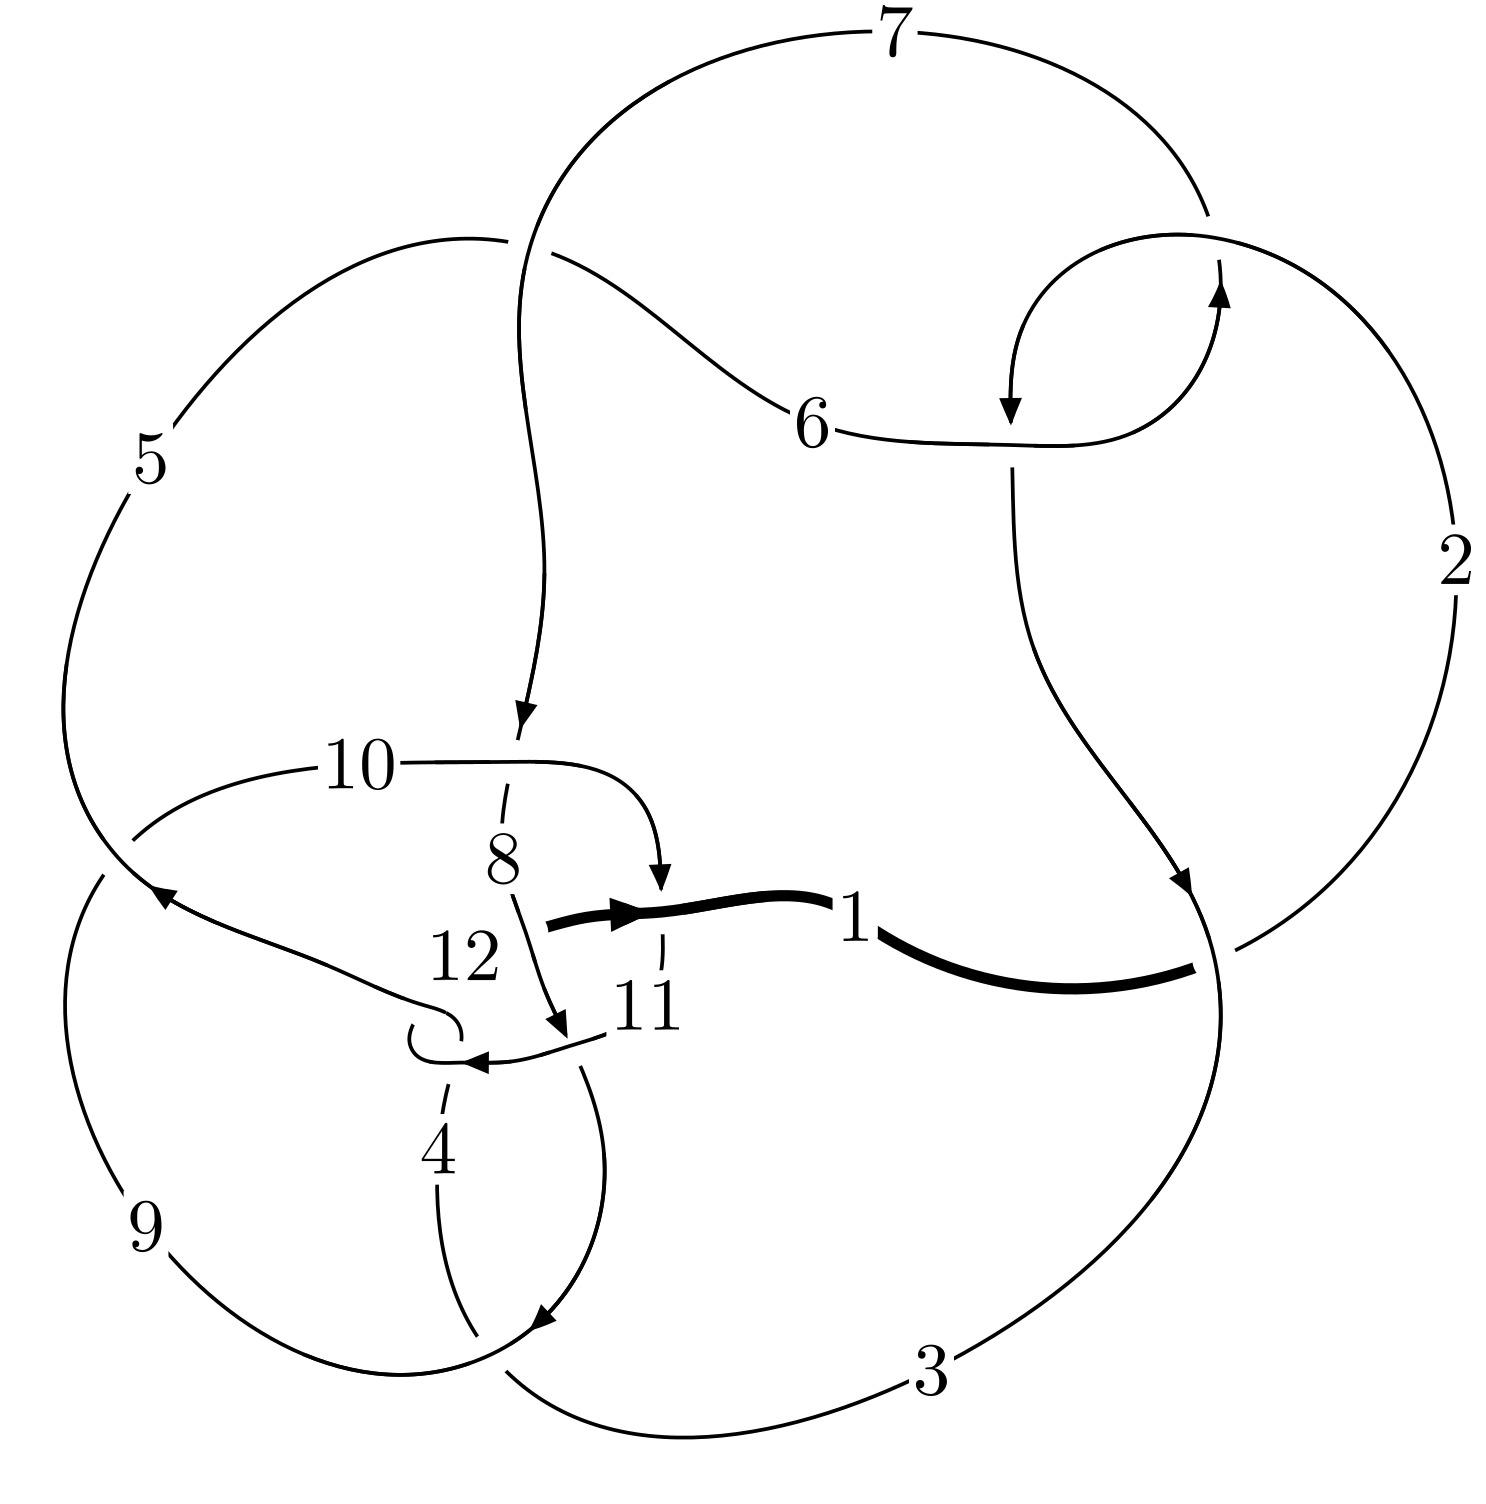
\includegraphics[width=112pt]{../../../GIT/diagram.site/Diagrams/png/2594_12n_0505.png}\\
\ \ \ A knot diagram\footnotemark}&
\allowdisplaybreaks
\textbf{Linearized knot diagam} \\
\cline{2-2}
 &
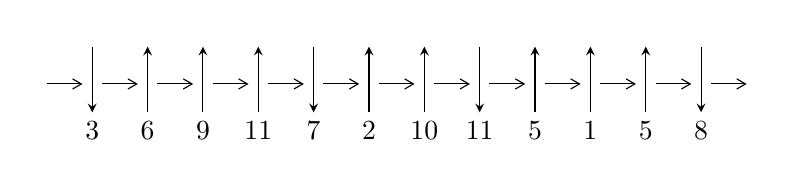
\begin{tikzpicture}[x=20pt, y=17pt]
	% nodes
	\node (C0) at (0, 0) {};
	\node (C1) at (1, 0) {};
	\node (C1U) at (1, +1) {};
	\node (C1D) at (1, -1) {3};

	\node (C2) at (2, 0) {};
	\node (C2U) at (2, +1) {};
	\node (C2D) at (2, -1) {6};

	\node (C3) at (3, 0) {};
	\node (C3U) at (3, +1) {};
	\node (C3D) at (3, -1) {9};

	\node (C4) at (4, 0) {};
	\node (C4U) at (4, +1) {};
	\node (C4D) at (4, -1) {11};

	\node (C5) at (5, 0) {};
	\node (C5U) at (5, +1) {};
	\node (C5D) at (5, -1) {7};

	\node (C6) at (6, 0) {};
	\node (C6U) at (6, +1) {};
	\node (C6D) at (6, -1) {2};

	\node (C7) at (7, 0) {};
	\node (C7U) at (7, +1) {};
	\node (C7D) at (7, -1) {10};

	\node (C8) at (8, 0) {};
	\node (C8U) at (8, +1) {};
	\node (C8D) at (8, -1) {11};

	\node (C9) at (9, 0) {};
	\node (C9U) at (9, +1) {};
	\node (C9D) at (9, -1) {5};

	\node (C10) at (10, 0) {};
	\node (C10U) at (10, +1) {};
	\node (C10D) at (10, -1) {1};

	\node (C11) at (11, 0) {};
	\node (C11U) at (11, +1) {};
	\node (C11D) at (11, -1) {5};

	\node (C12) at (12, 0) {};
	\node (C12U) at (12, +1) {};
	\node (C12D) at (12, -1) {8};
	\node (C13) at (13, 0) {};

	% arrows
	\draw[->,>={angle 60}]
	(C0) edge (C1) (C1) edge (C2) (C2) edge (C3) (C3) edge (C4) (C4) edge (C5) (C5) edge (C6) (C6) edge (C7) (C7) edge (C8) (C8) edge (C9) (C9) edge (C10) (C10) edge (C11) (C11) edge (C12) (C12) edge (C13) ;	\draw[->,>=stealth]
	(C1U) edge (C1D) (C2D) edge (C2U) (C3D) edge (C3U) (C4D) edge (C4U) (C5U) edge (C5D) (C6D) edge (C6U) (C7D) edge (C7U) (C8U) edge (C8D) (C9D) edge (C9U) (C10D) edge (C10U) (C11D) edge (C11U) (C12U) edge (C12D) ;
	\end{tikzpicture} \\
\hhline{~~} \\& 
\textbf{Solving Sequence} \\ \cline{2-2} 
 &
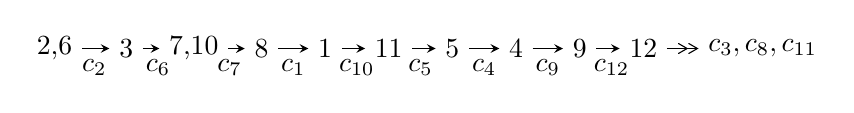
\begin{tikzpicture}[x=23pt, y=7pt]
	% node
	\node (A0) at (-1/8, 0) {2,6};
	\node (A1) at (1, 0) {3};
	\node (A2) at (33/16, 0) {7,10};
	\node (A3) at (25/8, 0) {8};
	\node (A4) at (33/8, 0) {1};
	\node (A5) at (41/8, 0) {11};
	\node (A6) at (49/8, 0) {5};
	\node (A7) at (57/8, 0) {4};
	\node (A8) at (65/8, 0) {9};
	\node (A9) at (73/8, 0) {12};
	\node (C1) at (1/2, -1) {$c_{2}$};
	\node (C2) at (3/2, -1) {$c_{6}$};
	\node (C3) at (21/8, -1) {$c_{7}$};
	\node (C4) at (29/8, -1) {$c_{1}$};
	\node (C5) at (37/8, -1) {$c_{10}$};
	\node (C6) at (45/8, -1) {$c_{5}$};
	\node (C7) at (53/8, -1) {$c_{4}$};
	\node (C8) at (61/8, -1) {$c_{9}$};
	\node (C9) at (69/8, -1) {$c_{12}$};
	\node (A10) at (11, 0) {$c_{3},c_{8},c_{11}$};

	% edge
	\draw[->,>=stealth]	
	(A0) edge (A1) (A1) edge (A2) (A2) edge (A3) (A3) edge (A4) (A4) edge (A5) (A5) edge (A6) (A6) edge (A7) (A7) edge (A8) (A8) edge (A9) ;
	\draw[->>,>={angle 60}]	
	(A9) edge (A10);
\end{tikzpicture} \\ 

\end{tabular} \\

\footnotetext{
The image of knot diagram is generated by the software ``\textbf{Draw programme}" developed by Andrew Bartholomew(\url{http://www.layer8.co.uk/maths/draw/index.htm\#Running-draw}), where we modified some parts for our purpose(\url{https://github.com/CATsTAILs/LinksPainter}).
}\phantom \\ \newline 
\centering \textbf{Ideals for irreducible components\footnotemark of $X_{\text{par}}$} 
 
\begin{align*}
I^u_{1}&=\langle 
-19 u^{31}+110 u^{30}+\cdots+b+35,\;-27 u^{31}+170 u^{30}+\cdots+2 a+74,\;u^{32}-6 u^{31}+\cdots+2 u+2\rangle \\
I^u_{2}&=\langle 
2 u^{14}+4 u^{12}- u^{11}+9 u^{10}+2 u^9+8 u^8+2 u^7+5 u^6+7 u^5+2 u^4+3 u^3-2 u^2+b+u-1,\\
\phantom{I^u_{2}}&\phantom{= \langle  }3 u^{14}- u^{13}+5 u^{12}-4 u^{11}+11 u^{10}-3 u^9+6 u^8-6 u^7- u^6-5 u^4-4 u^3-11 u^2+2 a-3 u-4,\\
\phantom{I^u_{2}}&\phantom{= \langle  }u^{15}- u^{14}+3 u^{13}-2 u^{12}+7 u^{11}-3 u^{10}+8 u^9+7 u^7+4 u^6+3 u^5+6 u^4+u^3+5 u^2+2\rangle \\
I^u_{3}&=\langle 
- u^{15}- u^{14}-2 u^{13}- u^{12}-4 u^{11}-2 u^{10}-4 u^9- u^8-4 u^7-2 u^5+u^2 a-2 u^3+a u+b+1,\\
\phantom{I^u_{3}}&\phantom{= \langle  }u^{15} a-5 u^{15}+\cdots-2 a+8,\\
\phantom{I^u_{3}}&\phantom{= \langle  }u^{16}+u^{15}+3 u^{14}+2 u^{13}+7 u^{12}+4 u^{11}+10 u^{10}+4 u^9+11 u^8+2 u^7+8 u^6+4 u^4-2 u^3-2 u-1\rangle \\
\\
\end{align*}
\raggedright * 3 irreducible components of $\dim_{\mathbb{C}}=0$, with total 79 representations.\\
\footnotetext{All coefficients of polynomials are rational numbers. But the coefficients are sometimes approximated in decimal forms when there is not enough margin.}
\newpage
\renewcommand{\arraystretch}{1}
\centering \section*{I. $I^u_{1}= \langle -19 u^{31}+110 u^{30}+\cdots+b+35,\;-27 u^{31}+170 u^{30}+\cdots+2 a+74,\;u^{32}-6 u^{31}+\cdots+2 u+2 \rangle$}
\flushleft \textbf{(i) Arc colorings}\\
\begin{tabular}{m{7pt} m{180pt} m{7pt} m{180pt} }
\flushright $a_{2}=$&$\begin{pmatrix}1\\0\end{pmatrix}$ \\
\flushright $a_{6}=$&$\begin{pmatrix}0\\u\end{pmatrix}$ \\
\flushright $a_{3}=$&$\begin{pmatrix}1\\- u^2\end{pmatrix}$ \\
\flushright $a_{7}=$&$\begin{pmatrix}u\\u\end{pmatrix}$ \\
\flushright $a_{10}=$&$\begin{pmatrix}\frac{27}{2} u^{31}-85 u^{30}+\cdots-58 u-37\\19 u^{31}-110 u^{30}+\cdots-45 u-35\end{pmatrix}$ \\
\flushright $a_{8}=$&$\begin{pmatrix}\frac{5}{2} u^{31}-15 u^{30}+\cdots-9 u-6\\2 u^{31}-13 u^{30}+\cdots-5 u-5\end{pmatrix}$ \\
\flushright $a_{1}=$&$\begin{pmatrix}u^2+1\\- u^4\end{pmatrix}$ \\
\flushright $a_{11}=$&$\begin{pmatrix}\frac{17}{2} u^{31}-50 u^{30}+\cdots-23 u-16\\10 u^{31}-55 u^{30}+\cdots-19 u-15\end{pmatrix}$ \\
\flushright $a_{5}=$&$\begin{pmatrix}u^3\\u^3+u\end{pmatrix}$ \\
\flushright $a_{4}=$&$\begin{pmatrix}-\frac{7}{2} u^{31}+16 u^{30}+\cdots- u+1\\- u^{31}+4 u^{29}+\cdots-11 u-5\end{pmatrix}$ \\
\flushright $a_{9}=$&$\begin{pmatrix}\frac{7}{2} u^{31}-16 u^{30}+\cdots+4 u-1\\-4 u^{31}+19 u^{30}+\cdots+2 u+3\end{pmatrix}$ \\
\flushright $a_{12}=$&$\begin{pmatrix}\frac{21}{2} u^{31}-65 u^{30}+\cdots-41 u-26\\16 u^{31}-89 u^{30}+\cdots-30 u-25\end{pmatrix}$\\&\end{tabular}
\flushleft \textbf{(ii) Obstruction class $= -1$}\\~\\
\flushleft \textbf{(iii) Cusp Shapes $= -16 u^{31}+83 u^{30}-289 u^{29}+706 u^{28}-1480 u^{27}+2622 u^{26}-4235 u^{25}+6012 u^{24}-7923 u^{23}+9315 u^{22}-10193 u^{21}+9679 u^{20}-8295 u^{19}+5507 u^{18}-2564 u^{17}-852 u^{16}+3101 u^{15}-4711 u^{14}+4654 u^{13}-4018 u^{12}+2292 u^{11}-761 u^{10}-695 u^9+1289 u^8-1440 u^7+990 u^6-534 u^5+157 u^4-23 u^3-26 u^2+2 u+16$}\\~\\
\newpage\renewcommand{\arraystretch}{1}
\flushleft \textbf{(iv) u-Polynomials at the component}\newline \\
\begin{tabular}{m{50pt}|m{274pt}}
Crossings & \hspace{64pt}u-Polynomials at each crossing \\
\hline $$\begin{aligned}c_{1},c_{5}\end{aligned}$$&$\begin{aligned}
&u^{32}+10 u^{31}+\cdots-12 u+4
\end{aligned}$\\
\hline $$\begin{aligned}c_{2},c_{6}\end{aligned}$$&$\begin{aligned}
&u^{32}-6 u^{31}+\cdots+2 u+2
\end{aligned}$\\
\hline $$\begin{aligned}c_{3},c_{4},c_{11}\end{aligned}$$&$\begin{aligned}
&u^{32}+u^{31}+\cdots-2 u+1
\end{aligned}$\\
\hline $$\begin{aligned}c_{7},c_{10}\end{aligned}$$&$\begin{aligned}
&u^{32}+3 u^{31}+\cdots-4 u+1
\end{aligned}$\\
\hline $$\begin{aligned}c_{8}\end{aligned}$$&$\begin{aligned}
&u^{32}-15 u^{31}+\cdots+330 u+50
\end{aligned}$\\
\hline $$\begin{aligned}c_{9}\end{aligned}$$&$\begin{aligned}
&u^{32}- u^{31}+\cdots+7 u+4
\end{aligned}$\\
\hline $$\begin{aligned}c_{12}\end{aligned}$$&$\begin{aligned}
&u^{32}+30 u^{31}+\cdots+983040 u+65536
\end{aligned}$\\
\hline
\end{tabular}\\~\\
\newpage\renewcommand{\arraystretch}{1}
\flushleft \textbf{(v) Riley Polynomials at the component}\newline \\
\begin{tabular}{m{50pt}|m{274pt}}
Crossings & \hspace{64pt}Riley Polynomials at each crossing \\
\hline $$\begin{aligned}c_{1},c_{5}\end{aligned}$$&$\begin{aligned}
&y^{32}+26 y^{31}+\cdots+336 y+16
\end{aligned}$\\
\hline $$\begin{aligned}c_{2},c_{6}\end{aligned}$$&$\begin{aligned}
&y^{32}+10 y^{31}+\cdots-12 y+4
\end{aligned}$\\
\hline $$\begin{aligned}c_{3},c_{4},c_{11}\end{aligned}$$&$\begin{aligned}
&y^{32}+45 y^{31}+\cdots+10 y+1
\end{aligned}$\\
\hline $$\begin{aligned}c_{7},c_{10}\end{aligned}$$&$\begin{aligned}
&y^{32}+5 y^{31}+\cdots-12 y+1
\end{aligned}$\\
\hline $$\begin{aligned}c_{8}\end{aligned}$$&$\begin{aligned}
&y^{32}-23 y^{31}+\cdots-127900 y+2500
\end{aligned}$\\
\hline $$\begin{aligned}c_{9}\end{aligned}$$&$\begin{aligned}
&y^{32}+9 y^{31}+\cdots+151 y+16
\end{aligned}$\\
\hline $$\begin{aligned}c_{12}\end{aligned}$$&$\begin{aligned}
&y^{32}-24 y^{30}+\cdots+4294967296 y+4294967296
\end{aligned}$\\
\hline
\end{tabular}\\~\\
\newpage\flushleft \textbf{(vi) Complex Volumes and Cusp Shapes}
$$\begin{array}{c|c|c}  
\text{Solutions to }I^u_{1}& \I (\text{vol} + \sqrt{-1}CS) & \text{Cusp shape}\\
 \hline 
\begin{aligned}
u &= -0.683755 + 0.852208 I \\
a &= \phantom{-}0.487406 + 0.002344 I \\
b &= -0.211885 + 0.982398 I\end{aligned}
 & \phantom{-}1.307790 - 0.204998 I & \phantom{-}8.20443 + 1.69179 I \\ \hline\begin{aligned}
u &= -0.683755 - 0.852208 I \\
a &= \phantom{-}0.487406 - 0.002344 I \\
b &= -0.211885 - 0.982398 I\end{aligned}
 & \phantom{-}1.307790 + 0.204998 I & \phantom{-}8.20443 - 1.69179 I \\ \hline\begin{aligned}
u &= \phantom{-}0.779459 + 0.786382 I \\
a &= -1.93860 - 1.52370 I \\
b &= -2.20178 - 0.35212 I\end{aligned}
 & \phantom{-}4.25545 - 1.80010 I & \phantom{-}6.28414 + 0.97881 I \\ \hline\begin{aligned}
u &= \phantom{-}0.779459 - 0.786382 I \\
a &= -1.93860 + 1.52370 I \\
b &= -2.20178 + 0.35212 I\end{aligned}
 & \phantom{-}4.25545 + 1.80010 I & \phantom{-}6.28414 - 0.97881 I \\ \hline\begin{aligned}
u &= -0.015119 + 0.891995 I \\
a &= \phantom{-}0.067954 + 0.845861 I \\
b &= -0.724294 + 0.722479 I\end{aligned}
 & -2.42371 + 1.04680 I & -1.12616 - 4.02159 I \\ \hline\begin{aligned}
u &= -0.015119 - 0.891995 I \\
a &= \phantom{-}0.067954 - 0.845861 I \\
b &= -0.724294 - 0.722479 I\end{aligned}
 & -2.42371 - 1.04680 I & -1.12616 + 4.02159 I \\ \hline\begin{aligned}
u &= -0.127331 + 0.878306 I \\
a &= \phantom{-}0.247595 - 1.216250 I \\
b &= \phantom{-}1.49574 - 0.49081 I\end{aligned}
 & -1.46153 - 3.39079 I & -2.40633 + 1.52334 I \\ \hline\begin{aligned}
u &= -0.127331 - 0.878306 I \\
a &= \phantom{-}0.247595 + 1.216250 I \\
b &= \phantom{-}1.49574 + 0.49081 I\end{aligned}
 & -1.46153 + 3.39079 I & -2.40633 - 1.52334 I \\ \hline\begin{aligned}
u &= \phantom{-}0.755098 + 0.457354 I \\
a &= \phantom{-}0.394809 - 0.506304 I \\
b &= \phantom{-}0.037452 - 0.291658 I\end{aligned}
 & \phantom{-}1.48779 + 0.53337 I & \phantom{-}11.99767 - 5.02878 I \\ \hline\begin{aligned}
u &= \phantom{-}0.755098 - 0.457354 I \\
a &= \phantom{-}0.394809 + 0.506304 I \\
b &= \phantom{-}0.037452 + 0.291658 I\end{aligned}
 & \phantom{-}1.48779 - 0.53337 I & \phantom{-}11.99767 + 5.02878 I\\
 \hline 
 \end{array}$$\newpage$$\begin{array}{c|c|c}  
\text{Solutions to }I^u_{1}& \I (\text{vol} + \sqrt{-1}CS) & \text{Cusp shape}\\
 \hline 
\begin{aligned}
u &= -0.686701 + 0.891793 I \\
a &= -0.391138 - 0.204261 I \\
b &= \phantom{-}0.574304 - 0.753738 I\end{aligned}
 & \phantom{-}1.18083 - 5.07845 I & \phantom{-}7.57041 + 6.17791 I \\ \hline\begin{aligned}
u &= -0.686701 - 0.891793 I \\
a &= -0.391138 + 0.204261 I \\
b &= \phantom{-}0.574304 + 0.753738 I\end{aligned}
 & \phantom{-}1.18083 + 5.07845 I & \phantom{-}7.57041 - 6.17791 I \\ \hline\begin{aligned}
u &= \phantom{-}0.884596 + 0.702295 I \\
a &= \phantom{-}1.55531 + 1.46424 I \\
b &= \phantom{-}1.71686 + 0.03149 I\end{aligned}
 & -2.61872 - 9.73264 I & \phantom{-}5.09358 + 3.95758 I \\ \hline\begin{aligned}
u &= \phantom{-}0.884596 - 0.702295 I \\
a &= \phantom{-}1.55531 - 1.46424 I \\
b &= \phantom{-}1.71686 - 0.03149 I\end{aligned}
 & -2.61872 + 9.73264 I & \phantom{-}5.09358 - 3.95758 I \\ \hline\begin{aligned}
u &= \phantom{-}0.719909 + 0.881933 I \\
a &= \phantom{-}0.89512 + 1.20915 I \\
b &= \phantom{-}1.34574 + 0.83709 I\end{aligned}
 & \phantom{-}1.47719 + 2.75279 I & \phantom{-}4.12705 - 2.54789 I \\ \hline\begin{aligned}
u &= \phantom{-}0.719909 - 0.881933 I \\
a &= \phantom{-}0.89512 - 1.20915 I \\
b &= \phantom{-}1.34574 - 0.83709 I\end{aligned}
 & \phantom{-}1.47719 - 2.75279 I & \phantom{-}4.12705 + 2.54789 I \\ \hline\begin{aligned}
u &= -0.232859 + 1.122020 I \\
a &= -0.327320 + 0.701313 I \\
b &= -1.47146 + 0.14327 I\end{aligned}
 & -10.17100 - 9.66976 I & -1.12021 + 6.59590 I \\ \hline\begin{aligned}
u &= -0.232859 - 1.122020 I \\
a &= -0.327320 - 0.701313 I \\
b &= -1.47146 - 0.14327 I\end{aligned}
 & -10.17100 + 9.66976 I & -1.12021 - 6.59590 I \\ \hline\begin{aligned}
u &= -0.815946 + 0.102282 I \\
a &= \phantom{-}0.523040 - 0.339256 I \\
b &= -0.678199 + 0.639931 I\end{aligned}
 & -6.02453 - 6.28492 I & \phantom{-}4.69674 + 5.01750 I \\ \hline\begin{aligned}
u &= -0.815946 - 0.102282 I \\
a &= \phantom{-}0.523040 + 0.339256 I \\
b &= -0.678199 - 0.639931 I\end{aligned}
 & -6.02453 + 6.28492 I & \phantom{-}4.69674 - 5.01750 I\\
 \hline 
 \end{array}$$\newpage$$\begin{array}{c|c|c}  
\text{Solutions to }I^u_{1}& \I (\text{vol} + \sqrt{-1}CS) & \text{Cusp shape}\\
 \hline 
\begin{aligned}
u &= -0.359796 + 1.131210 I \\
a &= -0.396826 - 0.243138 I \\
b &= \phantom{-}0.159308 - 0.964091 I\end{aligned}
 & -9.40796 + 2.11722 I & -1.44983 - 2.28702 I \\ \hline\begin{aligned}
u &= -0.359796 - 1.131210 I \\
a &= -0.396826 + 0.243138 I \\
b &= \phantom{-}0.159308 + 0.964091 I\end{aligned}
 & -9.40796 - 2.11722 I & -1.44983 + 2.28702 I \\ \hline\begin{aligned}
u &= \phantom{-}0.738924 + 0.951964 I \\
a &= -1.23531 - 2.20933 I \\
b &= -2.36280 - 1.86645 I\end{aligned}
 & \phantom{-}3.74678 + 7.53753 I & \phantom{-}5.07954 - 6.16050 I \\ \hline\begin{aligned}
u &= \phantom{-}0.738924 - 0.951964 I \\
a &= -1.23531 + 2.20933 I \\
b &= -2.36280 + 1.86645 I\end{aligned}
 & \phantom{-}3.74678 - 7.53753 I & \phantom{-}5.07954 + 6.16050 I \\ \hline\begin{aligned}
u &= \phantom{-}0.908160 + 0.896082 I \\
a &= \phantom{-}0.386593 + 0.792958 I \\
b &= \phantom{-}0.922704 + 0.420064 I\end{aligned}
 & \phantom{-}0.14826 + 3.30667 I & \phantom{-}11.82122 - 5.07419 I \\ \hline\begin{aligned}
u &= \phantom{-}0.908160 - 0.896082 I \\
a &= \phantom{-}0.386593 - 0.792958 I \\
b &= \phantom{-}0.922704 - 0.420064 I\end{aligned}
 & \phantom{-}0.14826 - 3.30667 I & \phantom{-}11.82122 + 5.07419 I \\ \hline\begin{aligned}
u &= \phantom{-}0.759511 + 1.036240 I \\
a &= \phantom{-}1.17713 + 1.86108 I \\
b &= \phantom{-}2.47993 + 1.70524 I\end{aligned}
 & -3.6530 + 15.8290 I & \phantom{-}3.56651 - 8.43512 I \\ \hline\begin{aligned}
u &= \phantom{-}0.759511 - 1.036240 I \\
a &= \phantom{-}1.17713 - 1.86108 I \\
b &= \phantom{-}2.47993 - 1.70524 I\end{aligned}
 & -3.6530 - 15.8290 I & \phantom{-}3.56651 + 8.43512 I \\ \hline\begin{aligned}
u &= \phantom{-}0.722062 + 1.151000 I \\
a &= -0.296051 - 0.228149 I \\
b &= -0.568245 - 0.196699 I\end{aligned}
 & -0.61804 + 5.20487 I & \phantom{-}14.5642 - 21.0319 I \\ \hline\begin{aligned}
u &= \phantom{-}0.722062 - 1.151000 I \\
a &= -0.296051 + 0.228149 I \\
b &= -0.568245 + 0.196699 I\end{aligned}
 & -0.61804 - 5.20487 I & \phantom{-}14.5642 + 21.0319 I\\
 \hline 
 \end{array}$$\newpage$$\begin{array}{c|c|c}  
\text{Solutions to }I^u_{1}& \I (\text{vol} + \sqrt{-1}CS) & \text{Cusp shape}\\
 \hline 
\begin{aligned}
u &= -0.346211 + 0.168211 I \\
a &= -0.14971 - 1.47915 I \\
b &= \phantom{-}0.486627 + 0.604920 I\end{aligned}
 & \phantom{-}0.56782 + 1.66520 I & \phantom{-}4.09705 - 5.80076 I \\ \hline\begin{aligned}
u &= -0.346211 - 0.168211 I \\
a &= -0.14971 + 1.47915 I \\
b &= \phantom{-}0.486627 - 0.604920 I\end{aligned}
 & \phantom{-}0.56782 - 1.66520 I & \phantom{-}4.09705 + 5.80076 I\\
 \hline 
 \end{array}$$\newpage\newpage\renewcommand{\arraystretch}{1}
\centering \section*{II. $I^u_{2}= \langle 2 u^{14}+4 u^{12}+\cdots+b-1,\;3 u^{14}- u^{13}+\cdots+2 a-4,\;u^{15}- u^{14}+\cdots+5 u^2+2 \rangle$}
\flushleft \textbf{(i) Arc colorings}\\
\begin{tabular}{m{7pt} m{180pt} m{7pt} m{180pt} }
\flushright $a_{2}=$&$\begin{pmatrix}1\\0\end{pmatrix}$ \\
\flushright $a_{6}=$&$\begin{pmatrix}0\\u\end{pmatrix}$ \\
\flushright $a_{3}=$&$\begin{pmatrix}1\\- u^2\end{pmatrix}$ \\
\flushright $a_{7}=$&$\begin{pmatrix}u\\u\end{pmatrix}$ \\
\flushright $a_{10}=$&$\begin{pmatrix}-\frac{3}{2} u^{14}+\frac{1}{2} u^{13}+\cdots+\frac{3}{2} u+2\\-2 u^{14}-4 u^{12}+\cdots- u+1\end{pmatrix}$ \\
\flushright $a_{8}=$&$\begin{pmatrix}\frac{1}{2} u^{14}+\frac{1}{2} u^{13}+\cdots-\frac{1}{2} u-1\\u^{14}+u^{13}+\cdots+u+1\end{pmatrix}$ \\
\flushright $a_{1}=$&$\begin{pmatrix}u^2+1\\- u^4\end{pmatrix}$ \\
\flushright $a_{11}=$&$\begin{pmatrix}-\frac{1}{2} u^{14}-\frac{1}{2} u^{13}+\cdots+\frac{1}{2} u-1\\- u^{14}-2 u^{12}+\cdots- u-1\end{pmatrix}$ \\
\flushright $a_{5}=$&$\begin{pmatrix}u^3\\u^3+u\end{pmatrix}$ \\
\flushright $a_{4}=$&$\begin{pmatrix}-\frac{1}{2} u^{14}-\frac{3}{2} u^{13}+\cdots-\frac{11}{2} u-4\\- u^{14}-2 u^{12}+\cdots-3 u-1\end{pmatrix}$ \\
\flushright $a_{9}=$&$\begin{pmatrix}\frac{1}{2} u^{14}-\frac{3}{2} u^{13}+\cdots+\frac{3}{2} u-2\\- u^9- u^7-2 u^5- u^4- u^2-1\end{pmatrix}$ \\
\flushright $a_{12}=$&$\begin{pmatrix}-\frac{3}{2} u^{14}+\frac{1}{2} u^{13}+\cdots+\frac{1}{2} u+1\\-2 u^{14}-4 u^{12}+\cdots-2 u-1\end{pmatrix}$\\&\end{tabular}
\flushleft \textbf{(ii) Obstruction class $= 1$}\\~\\
\flushleft \textbf{(iii) Cusp Shapes $= 4 u^{14}-6 u^{13}+12 u^{12}-12 u^{11}+24 u^{10}-24 u^9+22 u^8-14 u^7+8 u^6-8 u^5-8 u^4- u^3-12 u^2+2 u-4$}\\~\\
\newpage\renewcommand{\arraystretch}{1}
\flushleft \textbf{(iv) u-Polynomials at the component}\newline \\
\begin{tabular}{m{50pt}|m{274pt}}
Crossings & \hspace{64pt}u-Polynomials at each crossing \\
\hline $$\begin{aligned}c_{1},c_{5}\end{aligned}$$&$\begin{aligned}
&u^{15}-5 u^{14}+\cdots-20 u+4
\end{aligned}$\\
\hline $$\begin{aligned}c_{2}\end{aligned}$$&$\begin{aligned}
&u^{15}- u^{14}+\cdots+5 u^2+2
\end{aligned}$\\
\hline $$\begin{aligned}c_{3},c_{11}\end{aligned}$$&$\begin{aligned}
&u^{15}- u^{14}+\cdots-3 u+1
\end{aligned}$\\
\hline $$\begin{aligned}c_{4}\end{aligned}$$&$\begin{aligned}
&u^{15}+u^{14}+\cdots-3 u-1
\end{aligned}$\\
\hline $$\begin{aligned}c_{6}\end{aligned}$$&$\begin{aligned}
&u^{15}+u^{14}+\cdots-5 u^2-2
\end{aligned}$\\
\hline $$\begin{aligned}c_{7},c_{10}\end{aligned}$$&$\begin{aligned}
&u^{15}+3 u^{14}+\cdots+3 u+1
\end{aligned}$\\
\hline $$\begin{aligned}c_{8}\end{aligned}$$&$\begin{aligned}
&u^{15}-12 u^{14}+\cdots+12 u-2
\end{aligned}$\\
\hline $$\begin{aligned}c_{9}\end{aligned}$$&$\begin{aligned}
&u^{15}+u^{14}+\cdots+u-1
\end{aligned}$\\
\hline $$\begin{aligned}c_{12}\end{aligned}$$&$\begin{aligned}
&u^{15}+3 u^{14}+\cdots+3 u+1
\end{aligned}$\\
\hline
\end{tabular}\\~\\
\newpage\renewcommand{\arraystretch}{1}
\flushleft \textbf{(v) Riley Polynomials at the component}\newline \\
\begin{tabular}{m{50pt}|m{274pt}}
Crossings & \hspace{64pt}Riley Polynomials at each crossing \\
\hline $$\begin{aligned}c_{1},c_{5}\end{aligned}$$&$\begin{aligned}
&y^{15}+13 y^{14}+\cdots+8 y-16
\end{aligned}$\\
\hline $$\begin{aligned}c_{2},c_{6}\end{aligned}$$&$\begin{aligned}
&y^{15}+5 y^{14}+\cdots-20 y-4
\end{aligned}$\\
\hline $$\begin{aligned}c_{3},c_{4},c_{11}\end{aligned}$$&$\begin{aligned}
&y^{15}+9 y^{14}+\cdots+y-1
\end{aligned}$\\
\hline $$\begin{aligned}c_{7},c_{10}\end{aligned}$$&$\begin{aligned}
&y^{15}-7 y^{14}+\cdots- y-1
\end{aligned}$\\
\hline $$\begin{aligned}c_{8}\end{aligned}$$&$\begin{aligned}
&y^{15}-16 y^{14}+\cdots-12 y-4
\end{aligned}$\\
\hline $$\begin{aligned}c_{9}\end{aligned}$$&$\begin{aligned}
&y^{15}+13 y^{14}+\cdots+9 y-1
\end{aligned}$\\
\hline $$\begin{aligned}c_{12}\end{aligned}$$&$\begin{aligned}
&y^{15}+y^{14}+\cdots+7 y-1
\end{aligned}$\\
\hline
\end{tabular}\\~\\
\newpage\flushleft \textbf{(vi) Complex Volumes and Cusp Shapes}
$$\begin{array}{c|c|c}  
\text{Solutions to }I^u_{2}& \I (\text{vol} + \sqrt{-1}CS) & \text{Cusp shape}\\
 \hline 
\begin{aligned}
u &= -0.280327 + 0.923287 I \\
a &= \phantom{-}0.052905 - 0.728078 I \\
b &= \phantom{-}1.075220 - 0.283109 I\end{aligned}
 & -0.70220 - 4.00075 I & \phantom{-}5.18084 + 7.73675 I \\ \hline\begin{aligned}
u &= -0.280327 - 0.923287 I \\
a &= \phantom{-}0.052905 + 0.728078 I \\
b &= \phantom{-}1.075220 + 0.283109 I\end{aligned}
 & -0.70220 + 4.00075 I & \phantom{-}5.18084 - 7.73675 I \\ \hline\begin{aligned}
u &= -0.571277 + 0.761420 I \\
a &= \phantom{-}0.483935 - 0.067367 I \\
b &= -0.043929 + 0.810898 I\end{aligned}
 & \phantom{-}0.370462 + 0.285171 I & \phantom{-}1.32756 - 0.80118 I \\ \hline\begin{aligned}
u &= -0.571277 - 0.761420 I \\
a &= \phantom{-}0.483935 + 0.067367 I \\
b &= -0.043929 - 0.810898 I\end{aligned}
 & \phantom{-}0.370462 - 0.285171 I & \phantom{-}1.32756 + 0.80118 I \\ \hline\begin{aligned}
u &= \phantom{-}0.692893 + 0.869031 I \\
a &= \phantom{-}2.38866 + 2.52848 I \\
b &= \phantom{-}3.15994 + 1.64676 I\end{aligned}
 & -4.59955 + 2.66562 I & \phantom{-}7.43536 - 3.52497 I \\ \hline\begin{aligned}
u &= \phantom{-}0.692893 - 0.869031 I \\
a &= \phantom{-}2.38866 - 2.52848 I \\
b &= \phantom{-}3.15994 - 1.64676 I\end{aligned}
 & -4.59955 - 2.66562 I & \phantom{-}7.43536 + 3.52497 I \\ \hline\begin{aligned}
u &= -0.877263\phantom{ +0.000000I} \\
a &= -0.247126\phantom{ +0.000000I} \\
b &= \phantom{-}0.406981\phantom{ +0.000000I}\end{aligned}
 & \phantom{-}1.99799\phantom{ +0.000000I} & \phantom{-}22.9980\phantom{ +0.000000I} \\ \hline\begin{aligned}
u &= \phantom{-}0.852657 + 0.760960 I \\
a &= -1.19418 - 1.44954 I \\
b &= -1.61952 - 0.38054 I\end{aligned}
 & \phantom{-}6.57862 - 2.60076 I & \phantom{-}11.64016 + 2.05519 I \\ \hline\begin{aligned}
u &= \phantom{-}0.852657 - 0.760960 I \\
a &= -1.19418 + 1.44954 I \\
b &= -1.61952 + 0.38054 I\end{aligned}
 & \phantom{-}6.57862 + 2.60076 I & \phantom{-}11.64016 - 2.05519 I \\ \hline\begin{aligned}
u &= \phantom{-}0.142705 + 0.800687 I \\
a &= -1.76224 + 0.77168 I \\
b &= -1.78689 - 0.41916 I\end{aligned}
 & -7.67025 + 0.63840 I & -0.866787 + 0.877859 I\\
 \hline 
 \end{array}$$\newpage$$\begin{array}{c|c|c}  
\text{Solutions to }I^u_{2}& \I (\text{vol} + \sqrt{-1}CS) & \text{Cusp shape}\\
 \hline 
\begin{aligned}
u &= \phantom{-}0.142705 - 0.800687 I \\
a &= -1.76224 - 0.77168 I \\
b &= -1.78689 + 0.41916 I\end{aligned}
 & -7.67025 - 0.63840 I & -0.866787 - 0.877859 I \\ \hline\begin{aligned}
u &= \phantom{-}0.769086 + 0.992896 I \\
a &= -1.22437 - 1.54363 I \\
b &= -2.24931 - 1.14168 I\end{aligned}
 & \phantom{-}5.85838 + 8.64297 I & \phantom{-}10.04873 - 7.11633 I \\ \hline\begin{aligned}
u &= \phantom{-}0.769086 - 0.992896 I \\
a &= -1.22437 + 1.54363 I \\
b &= -2.24931 + 1.14168 I\end{aligned}
 & \phantom{-}5.85838 - 8.64297 I & \phantom{-}10.04873 + 7.11633 I \\ \hline\begin{aligned}
u &= -0.667106 + 1.077180 I \\
a &= -0.121148 - 0.106125 I \\
b &= \phantom{-}0.261000 - 0.309723 I\end{aligned}
 & -0.83445 - 4.97703 I & -3.26494 + 1.29068 I \\ \hline\begin{aligned}
u &= -0.667106 - 1.077180 I \\
a &= -0.121148 + 0.106125 I \\
b &= \phantom{-}0.261000 + 0.309723 I\end{aligned}
 & -0.83445 + 4.97703 I & -3.26494 - 1.29068 I\\
 \hline 
 \end{array}$$\newpage\newpage\renewcommand{\arraystretch}{1}
\centering \section*{III. $I^u_{3}= \langle - u^{15}- u^{14}+\cdots+b+1,\;u^{15} a-5 u^{15}+\cdots-2 a+8,\;u^{16}+u^{15}+\cdots-2 u-1 \rangle$}
\flushleft \textbf{(i) Arc colorings}\\
\begin{tabular}{m{7pt} m{180pt} m{7pt} m{180pt} }
\flushright $a_{2}=$&$\begin{pmatrix}1\\0\end{pmatrix}$ \\
\flushright $a_{6}=$&$\begin{pmatrix}0\\u\end{pmatrix}$ \\
\flushright $a_{3}=$&$\begin{pmatrix}1\\- u^2\end{pmatrix}$ \\
\flushright $a_{7}=$&$\begin{pmatrix}u\\u\end{pmatrix}$ \\
\flushright $a_{10}=$&$\begin{pmatrix}a\\u^{15}+u^{14}+\cdots- a u-1\end{pmatrix}$ \\
\flushright $a_{8}=$&$\begin{pmatrix}u^{15}+u^{14}+\cdots- a+2\\- u^{13} a+2 u^{13}+\cdots+a u+1\end{pmatrix}$ \\
\flushright $a_{1}=$&$\begin{pmatrix}u^2+1\\- u^4\end{pmatrix}$ \\
\flushright $a_{11}=$&$\begin{pmatrix}- u^{15}- u^{14}+\cdots+a-1\\-2 u^{13}-2 u^{12}+\cdots+u-1\end{pmatrix}$ \\
\flushright $a_{5}=$&$\begin{pmatrix}u^3\\u^3+u\end{pmatrix}$ \\
\flushright $a_{4}=$&$\begin{pmatrix}3 u^{15}+u^{14}+\cdots+a-5\\u^{15}+u^{14}+\cdots+a u-1\end{pmatrix}$ \\
\flushright $a_{9}=$&$\begin{pmatrix}- u^{15}- u^{14}+\cdots+u^3+a\\-2 u^{13}-2 u^{12}+\cdots+u-1\end{pmatrix}$ \\
\flushright $a_{12}=$&$\begin{pmatrix}- u^{15}- u^{14}+\cdots+a-1\\u^{13} a-2 u^{13}+\cdots- a u-1\end{pmatrix}$\\&\end{tabular}
\flushleft \textbf{(ii) Obstruction class $= -1$}\\~\\
\flushleft \textbf{(iii) Cusp Shapes $= -4 u^{15}-8 u^{13}+4 u^{12}-20 u^{11}+8 u^{10}-24 u^9+16 u^8-28 u^7+20 u^6-20 u^5+16 u^4-12 u^3+12 u^2+2$}\\~\\
\newpage\renewcommand{\arraystretch}{1}
\flushleft \textbf{(iv) u-Polynomials at the component}\newline \\
\begin{tabular}{m{50pt}|m{274pt}}
Crossings & \hspace{64pt}u-Polynomials at each crossing \\
\hline $$\begin{aligned}c_{1},c_{5}\end{aligned}$$&$\begin{aligned}
&(u^{16}+5 u^{15}+\cdots-4 u+1)^{2}
\end{aligned}$\\
\hline $$\begin{aligned}c_{2},c_{6}\end{aligned}$$&$\begin{aligned}
&(u^{16}+u^{15}+\cdots-2 u-1)^{2}
\end{aligned}$\\
\hline $$\begin{aligned}c_{3},c_{4},c_{11}\end{aligned}$$&$\begin{aligned}
&u^{32}+u^{31}+\cdots-27 u+286
\end{aligned}$\\
\hline $$\begin{aligned}c_{7},c_{10}\end{aligned}$$&$\begin{aligned}
&u^{32}+13 u^{31}+\cdots-41 u-2
\end{aligned}$\\
\hline $$\begin{aligned}c_{8}\end{aligned}$$&$\begin{aligned}
&(u^{16}+13 u^{15}+\cdots+44 u-7)^{2}
\end{aligned}$\\
\hline $$\begin{aligned}c_{9}\end{aligned}$$&$\begin{aligned}
&u^{32}- u^{31}+\cdots-5662 u-169
\end{aligned}$\\
\hline $$\begin{aligned}c_{12}\end{aligned}$$&$\begin{aligned}
&(u-1)^{32}
\end{aligned}$\\
\hline
\end{tabular}\\~\\
\newpage\renewcommand{\arraystretch}{1}
\flushleft \textbf{(v) Riley Polynomials at the component}\newline \\
\begin{tabular}{m{50pt}|m{274pt}}
Crossings & \hspace{64pt}Riley Polynomials at each crossing \\
\hline $$\begin{aligned}c_{1},c_{5}\end{aligned}$$&$\begin{aligned}
&(y^{16}+13 y^{15}+\cdots-48 y+1)^{2}
\end{aligned}$\\
\hline $$\begin{aligned}c_{2},c_{6}\end{aligned}$$&$\begin{aligned}
&(y^{16}+5 y^{15}+\cdots-4 y+1)^{2}
\end{aligned}$\\
\hline $$\begin{aligned}c_{3},c_{4},c_{11}\end{aligned}$$&$\begin{aligned}
&y^{32}+39 y^{31}+\cdots+1346331 y+81796
\end{aligned}$\\
\hline $$\begin{aligned}c_{7},c_{10}\end{aligned}$$&$\begin{aligned}
&y^{32}-9 y^{31}+\cdots-53 y+4
\end{aligned}$\\
\hline $$\begin{aligned}c_{8}\end{aligned}$$&$\begin{aligned}
&(y^{16}-31 y^{15}+\cdots-704 y+49)^{2}
\end{aligned}$\\
\hline $$\begin{aligned}c_{9}\end{aligned}$$&$\begin{aligned}
&y^{32}+19 y^{31}+\cdots-25101866 y+28561
\end{aligned}$\\
\hline $$\begin{aligned}c_{12}\end{aligned}$$&$\begin{aligned}
&(y-1)^{32}
\end{aligned}$\\
\hline
\end{tabular}\\~\\
\newpage\flushleft \textbf{(vi) Complex Volumes and Cusp Shapes}
$$\begin{array}{c|c|c}  
\text{Solutions to }I^u_{3}& \I (\text{vol} + \sqrt{-1}CS) & \text{Cusp shape}\\
 \hline 
\begin{aligned}
u &= \phantom{-}0.254861 + 1.023380 I \\
a &= \phantom{-}0.166841 + 0.823281 I \\
b &= \phantom{-}0.776440 + 0.691048 I\end{aligned}
 & -1.88017 + 3.12434 I & -2.05940 - 3.66013 I \\ \hline\begin{aligned}
u &= \phantom{-}0.254861 + 1.023380 I \\
a &= \phantom{-}0.013723 - 0.175484 I \\
b &= -0.878070 + 0.201017 I\end{aligned}
 & -1.88017 + 3.12434 I & -2.05940 - 3.66013 I \\ \hline\begin{aligned}
u &= \phantom{-}0.254861 - 1.023380 I \\
a &= \phantom{-}0.166841 - 0.823281 I \\
b &= \phantom{-}0.776440 - 0.691048 I\end{aligned}
 & -1.88017 - 3.12434 I & -2.05940 + 3.66013 I \\ \hline\begin{aligned}
u &= \phantom{-}0.254861 - 1.023380 I \\
a &= \phantom{-}0.013723 + 0.175484 I \\
b &= -0.878070 - 0.201017 I\end{aligned}
 & -1.88017 - 3.12434 I & -2.05940 + 3.66013 I \\ \hline\begin{aligned}
u &= \phantom{-}0.750689 + 0.759364 I \\
a &= \phantom{-}0.24992 + 1.51155 I \\
b &= -0.196588 + 0.591384 I\end{aligned}
 & -2.97876 - 0.48968 I & \phantom{-}2.35607 + 1.43137 I \\ \hline\begin{aligned}
u &= \phantom{-}0.750689 + 0.759364 I \\
a &= -0.69577 + 1.84479 I \\
b &= \phantom{-}1.13391 + 2.14189 I\end{aligned}
 & -2.97876 - 0.48968 I & \phantom{-}2.35607 + 1.43137 I \\ \hline\begin{aligned}
u &= \phantom{-}0.750689 - 0.759364 I \\
a &= \phantom{-}0.24992 - 1.51155 I \\
b &= -0.196588 - 0.591384 I\end{aligned}
 & -2.97876 + 0.48968 I & \phantom{-}2.35607 - 1.43137 I \\ \hline\begin{aligned}
u &= \phantom{-}0.750689 - 0.759364 I \\
a &= -0.69577 - 1.84479 I \\
b &= \phantom{-}1.13391 - 2.14189 I\end{aligned}
 & -2.97876 + 0.48968 I & \phantom{-}2.35607 - 1.43137 I \\ \hline\begin{aligned}
u &= -0.099165 + 0.920214 I \\
a &= \phantom{-}0.057858 + 1.349270 I \\
b &= \phantom{-}0.976760 - 0.554322 I\end{aligned}
 & -8.46679 - 1.52971 I & -6.72737 + 5.08772 I \\ \hline\begin{aligned}
u &= -0.099165 + 0.920214 I \\
a &= -1.95590 - 1.06565 I \\
b &= -2.68988 - 1.32943 I\end{aligned}
 & -8.46679 - 1.52971 I & -6.72737 + 5.08772 I\\
 \hline 
 \end{array}$$\newpage$$\begin{array}{c|c|c}  
\text{Solutions to }I^u_{3}& \I (\text{vol} + \sqrt{-1}CS) & \text{Cusp shape}\\
 \hline 
\begin{aligned}
u &= -0.099165 - 0.920214 I \\
a &= \phantom{-}0.057858 - 1.349270 I \\
b &= \phantom{-}0.976760 + 0.554322 I\end{aligned}
 & -8.46679 + 1.52971 I & -6.72737 - 5.08772 I \\ \hline\begin{aligned}
u &= -0.099165 - 0.920214 I \\
a &= -1.95590 + 1.06565 I \\
b &= -2.68988 + 1.32943 I\end{aligned}
 & -8.46679 + 1.52971 I & -6.72737 - 5.08772 I \\ \hline\begin{aligned}
u &= -0.665350 + 0.873267 I \\
a &= \phantom{-}2.10683 - 2.08817 I \\
b &= \phantom{-}2.12567 - 2.22461 I\end{aligned}
 & -5.56244 - 2.57669 I & -3.30756 + 2.71681 I \\ \hline\begin{aligned}
u &= -0.665350 + 0.873267 I \\
a &= -2.36347 + 2.91711 I \\
b &= -3.72419 + 1.41589 I\end{aligned}
 & -5.56244 - 2.57669 I & -3.30756 + 2.71681 I \\ \hline\begin{aligned}
u &= -0.665350 - 0.873267 I \\
a &= \phantom{-}2.10683 + 2.08817 I \\
b &= \phantom{-}2.12567 + 2.22461 I\end{aligned}
 & -5.56244 + 2.57669 I & -3.30756 - 2.71681 I \\ \hline\begin{aligned}
u &= -0.665350 - 0.873267 I \\
a &= -2.36347 - 2.91711 I \\
b &= -3.72419 - 1.41589 I\end{aligned}
 & -5.56244 + 2.57669 I & -3.30756 - 2.71681 I \\ \hline\begin{aligned}
u &= -0.847960 + 0.745397 I \\
a &= -1.07862 + 1.20524 I \\
b &= -1.287070 + 0.510746 I\end{aligned}
 & \phantom{-}5.32084 + 2.28357 I & \phantom{-}3.92472 - 0.30826 I \\ \hline\begin{aligned}
u &= -0.847960 + 0.745397 I \\
a &= \phantom{-}1.17114 - 1.41311 I \\
b &= \phantom{-}1.61121 - 0.11458 I\end{aligned}
 & \phantom{-}5.32084 + 2.28357 I & \phantom{-}3.92472 - 0.30826 I \\ \hline\begin{aligned}
u &= -0.847960 - 0.745397 I \\
a &= -1.07862 - 1.20524 I \\
b &= -1.287070 - 0.510746 I\end{aligned}
 & \phantom{-}5.32084 - 2.28357 I & \phantom{-}3.92472 + 0.30826 I \\ \hline\begin{aligned}
u &= -0.847960 - 0.745397 I \\
a &= \phantom{-}1.17114 + 1.41311 I \\
b &= \phantom{-}1.61121 + 0.11458 I\end{aligned}
 & \phantom{-}5.32084 - 2.28357 I & \phantom{-}3.92472 + 0.30826 I\\
 \hline 
 \end{array}$$\newpage$$\begin{array}{c|c|c}  
\text{Solutions to }I^u_{3}& \I (\text{vol} + \sqrt{-1}CS) & \text{Cusp shape}\\
 \hline 
\begin{aligned}
u &= \phantom{-}0.716556 + 0.957138 I \\
a &= \phantom{-}1.273310 - 0.043889 I \\
b &= \phantom{-}2.08123 + 0.26719 I\end{aligned}
 & -3.57736 + 6.07197 I & \phantom{-}0.61575 - 7.02814 I \\ \hline\begin{aligned}
u &= \phantom{-}0.716556 + 0.957138 I \\
a &= \phantom{-}2.17649 - 0.07224 I \\
b &= \phantom{-}1.73170 - 1.82727 I\end{aligned}
 & -3.57736 + 6.07197 I & \phantom{-}0.61575 - 7.02814 I \\ \hline\begin{aligned}
u &= \phantom{-}0.716556 - 0.957138 I \\
a &= \phantom{-}1.273310 + 0.043889 I \\
b &= \phantom{-}2.08123 - 0.26719 I\end{aligned}
 & -3.57736 - 6.07197 I & \phantom{-}0.61575 + 7.02814 I \\ \hline\begin{aligned}
u &= \phantom{-}0.716556 - 0.957138 I \\
a &= \phantom{-}2.17649 + 0.07224 I \\
b &= \phantom{-}1.73170 + 1.82727 I\end{aligned}
 & -3.57736 - 6.07197 I & \phantom{-}0.61575 + 7.02814 I \\ \hline\begin{aligned}
u &= -0.761782 + 1.000110 I \\
a &= -1.07483 + 1.36444 I \\
b &= -1.75138 + 1.17047 I\end{aligned}
 & \phantom{-}4.53468 - 8.28859 I & \phantom{-}2.57708 + 5.27135 I \\ \hline\begin{aligned}
u &= -0.761782 + 1.000110 I \\
a &= \phantom{-}1.03895 - 1.57028 I \\
b &= \phantom{-}2.28316 - 1.19066 I\end{aligned}
 & \phantom{-}4.53468 - 8.28859 I & \phantom{-}2.57708 + 5.27135 I \\ \hline\begin{aligned}
u &= -0.761782 - 1.000110 I \\
a &= -1.07483 - 1.36444 I \\
b &= -1.75138 - 1.17047 I\end{aligned}
 & \phantom{-}4.53468 + 8.28859 I & \phantom{-}2.57708 - 5.27135 I \\ \hline\begin{aligned}
u &= -0.761782 - 1.000110 I \\
a &= \phantom{-}1.03895 + 1.57028 I \\
b &= \phantom{-}2.28316 + 1.19066 I\end{aligned}
 & \phantom{-}4.53468 + 8.28859 I & \phantom{-}2.57708 - 5.27135 I \\ \hline\begin{aligned}
u &= \phantom{-}0.689113\phantom{ +0.000000I} \\
a &= \phantom{-}0.757498\phantom{ +0.000000I} \\
b &= -0.278882\phantom{ +0.000000I}\end{aligned}
 & \phantom{-}1.42684\phantom{ +0.000000I} & \phantom{-}4.14780\phantom{ +0.000000I} \\ \hline\begin{aligned}
u &= \phantom{-}0.689113\phantom{ +0.000000I} \\
a &= \phantom{-}0.117305\phantom{ +0.000000I} \\
b &= \phantom{-}0.466296\phantom{ +0.000000I}\end{aligned}
 & \phantom{-}1.42684\phantom{ +0.000000I} & \phantom{-}4.14780\phantom{ +0.000000I}\\
 \hline 
 \end{array}$$\newpage$$\begin{array}{c|c|c}  
\text{Solutions to }I^u_{3}& \I (\text{vol} + \sqrt{-1}CS) & \text{Cusp shape}\\
 \hline 
\begin{aligned}
u &= -0.384812\phantom{ +0.000000I} \\
a &= \phantom{-}1.47613 + 2.83234 I \\
b &= -0.786617 + 0.670506 I\end{aligned}
 & -5.81564\phantom{ +0.000000I} & \phantom{-}5.09360\phantom{ +0.000000I} \\ \hline\begin{aligned}
u &= -0.384812\phantom{ +0.000000I} \\
a &= \phantom{-}1.47613 - 2.83234 I \\
b &= -0.786617 - 0.670506 I\end{aligned}
 & -5.81564\phantom{ +0.000000I} & \phantom{-}5.09360\phantom{ +0.000000I}\\
 \hline 
 \end{array}$$\newpage
\newpage\renewcommand{\arraystretch}{1}
\centering \section*{ IV. u-Polynomials}
\begin{tabular}{m{50pt}|m{274pt}}
Crossings & \hspace{64pt}u-Polynomials at each crossing \\
\hline $$\begin{aligned}c_{1},c_{5}\end{aligned}$$&$\begin{aligned}
&(u^{15}-5 u^{14}+\cdots-20 u+4)(u^{16}+5 u^{15}+\cdots-4 u+1)^{2}\\
&\cdot(u^{32}+10 u^{31}+\cdots-12 u+4)
\end{aligned}$\\
\hline $$\begin{aligned}c_{2}\end{aligned}$$&$\begin{aligned}
&(u^{15}- u^{14}+\cdots+5 u^2+2)(u^{16}+u^{15}+\cdots-2 u-1)^{2}\\
&\cdot(u^{32}-6 u^{31}+\cdots+2 u+2)
\end{aligned}$\\
\hline $$\begin{aligned}c_{3},c_{11}\end{aligned}$$&$\begin{aligned}
&(u^{15}- u^{14}+\cdots-3 u+1)(u^{32}+u^{31}+\cdots-27 u+286)\\
&\cdot(u^{32}+u^{31}+\cdots-2 u+1)
\end{aligned}$\\
\hline $$\begin{aligned}c_{4}\end{aligned}$$&$\begin{aligned}
&(u^{15}+u^{14}+\cdots-3 u-1)(u^{32}+u^{31}+\cdots-27 u+286)\\
&\cdot(u^{32}+u^{31}+\cdots-2 u+1)
\end{aligned}$\\
\hline $$\begin{aligned}c_{6}\end{aligned}$$&$\begin{aligned}
&(u^{15}+u^{14}+\cdots-5 u^2-2)(u^{16}+u^{15}+\cdots-2 u-1)^{2}\\
&\cdot(u^{32}-6 u^{31}+\cdots+2 u+2)
\end{aligned}$\\
\hline $$\begin{aligned}c_{7},c_{10}\end{aligned}$$&$\begin{aligned}
&(u^{15}+3 u^{14}+\cdots+3 u+1)(u^{32}+3 u^{31}+\cdots-4 u+1)\\
&\cdot(u^{32}+13 u^{31}+\cdots-41 u-2)
\end{aligned}$\\
\hline $$\begin{aligned}c_{8}\end{aligned}$$&$\begin{aligned}
&(u^{15}-12 u^{14}+\cdots+12 u-2)(u^{16}+13 u^{15}+\cdots+44 u-7)^{2}\\
&\cdot(u^{32}-15 u^{31}+\cdots+330 u+50)
\end{aligned}$\\
\hline $$\begin{aligned}c_{9}\end{aligned}$$&$\begin{aligned}
&(u^{15}+u^{14}+\cdots+u-1)(u^{32}- u^{31}+\cdots+7 u+4)\\
&\cdot(u^{32}- u^{31}+\cdots-5662 u-169)
\end{aligned}$\\
\hline $$\begin{aligned}c_{12}\end{aligned}$$&$\begin{aligned}
&((u-1)^{32})(u^{15}+3 u^{14}+\cdots+3 u+1)\\
&\cdot(u^{32}+30 u^{31}+\cdots+983040 u+65536)
\end{aligned}$\\
\hline
\end{tabular}\newpage\renewcommand{\arraystretch}{1}
\centering \section*{ V. Riley Polynomials}
\begin{tabular}{m{50pt}|m{274pt}}
Crossings & \hspace{64pt}Riley Polynomials at each crossing \\
\hline $$\begin{aligned}c_{1},c_{5}\end{aligned}$$&$\begin{aligned}
&(y^{15}+13 y^{14}+\cdots+8 y-16)(y^{16}+13 y^{15}+\cdots-48 y+1)^{2}\\
&\cdot(y^{32}+26 y^{31}+\cdots+336 y+16)
\end{aligned}$\\
\hline $$\begin{aligned}c_{2},c_{6}\end{aligned}$$&$\begin{aligned}
&(y^{15}+5 y^{14}+\cdots-20 y-4)(y^{16}+5 y^{15}+\cdots-4 y+1)^{2}\\
&\cdot(y^{32}+10 y^{31}+\cdots-12 y+4)
\end{aligned}$\\
\hline $$\begin{aligned}c_{3},c_{4},c_{11}\end{aligned}$$&$\begin{aligned}
&(y^{15}+9 y^{14}+\cdots+y-1)(y^{32}+39 y^{31}+\cdots+1346331 y+81796)\\
&\cdot(y^{32}+45 y^{31}+\cdots+10 y+1)
\end{aligned}$\\
\hline $$\begin{aligned}c_{7},c_{10}\end{aligned}$$&$\begin{aligned}
&(y^{15}-7 y^{14}+\cdots- y-1)(y^{32}-9 y^{31}+\cdots-53 y+4)\\
&\cdot(y^{32}+5 y^{31}+\cdots-12 y+1)
\end{aligned}$\\
\hline $$\begin{aligned}c_{8}\end{aligned}$$&$\begin{aligned}
&(y^{15}-16 y^{14}+\cdots-12 y-4)(y^{16}-31 y^{15}+\cdots-704 y+49)^{2}\\
&\cdot(y^{32}-23 y^{31}+\cdots-127900 y+2500)
\end{aligned}$\\
\hline $$\begin{aligned}c_{9}\end{aligned}$$&$\begin{aligned}
&(y^{15}+13 y^{14}+\cdots+9 y-1)(y^{32}+9 y^{31}+\cdots+151 y+16)\\
&\cdot(y^{32}+19 y^{31}+\cdots-25101866 y+28561)
\end{aligned}$\\
\hline $$\begin{aligned}c_{12}\end{aligned}$$&$\begin{aligned}
&((y-1)^{32})(y^{15}+y^{14}+\cdots+7 y-1)\\
&\cdot(y^{32}-24 y^{30}+\cdots+4294967296 y+4294967296)
\end{aligned}$\\
\hline
\end{tabular}
\vskip 2pc
\end{document}